
\chapter{Plane and Teaching of Coordinate Geometry in the Upper
  School}

\begin{center}
{\em By~} T. A. A. BROADBENT
\end{center}

\setcounter{pageoriginal}{28}
Some\pageoriginale time ago, I had a most instuctive discussion with a friend of
mine, a man of considerable experience as a teacher and examiner of
mathematics. The discussion arose from an idle question of mine :
whatm in his opinion, were the examination black spots, the topics
least efficiently handled by examination candidates. As far as the
upper school and first year university level was concerned, his answer
was given without hesitation and with great definiteness : statics and
coordinate geometry. From this we were very naturally led to ask why
this should be so, for the wise teacher can learn a great deal about
his teaching by studying scripts written by examiness.

It was possible, my friend thought, to give a clear-cut answer to this
further question, at any rate as regards statics. Here, he said, the
candidates were generally well acquainted with the principles to be
applied, but failed to apply them accurately, usually because of their
inability to isolate and to specify with precision the particular
system to which these principles are to be applied. This vagueness, he
thought, lay at the root of the confusion which is apt to show itself
at a later stage, when the energy of a system is under consideration.

When we turned to coordinate geometry, the question as to why this is
a black spot was not so easy to answer in simple terms. It did,
however, appear that one strong reason is that here the candidates are
not aware that there are any principles to be applied. They do not
search for the basic principle underlying the problem, they do not
look for a main clue to guide them from question to answer, they have
not learned that they should, at this level, see in the mind the whole
plane of the solution before anything in the way of detailed algebraic
calculation is put down on paper. Instead, they impatiently rush to
convert any geometric fact into some algebraic form, and then, having
accumulated a mass of uncorrelated and repulsive
equations,\pageoriginale they may bravely but blindly attempt to
manipulate these, usually plunging still deeper into the morass, or,
with more discretion, they may turn their backs on the chaos and pass
on to the next question.

Let me take a very childish but instructive instance, provided by a
question set in a recent examination for school children. ``The point
$A$ has coordinates $(2,1)$, the point $B$ has coordinates $(3,4)$;
find the coordinates of the point $C$ such that $B$ is the midpoint of
$AC$''. A proportion---not a large proportion, but still a significant
proportion---of the candidates proceeded thus. First they calculated
the length $AB$ by the Pythagorean formula; they then constructed the
equation to the circle of centre $B$ and radius $A,B$, and the
equation to the straight line $AB$; the they solved---or attempted to
solve---these two equations, thus to obtain the coordinates of $C$, as
well, of course, as those of $A$.

A first comment, perhaps superficial but not without value, is that
whatever the merits or demerits of this process as a piece of
mathematics, the luxuriance of its arithmetical requirements is
certain to multiply the possibility of mere arithmetic error. Each
step is one over which even a fairly sophisticated child may
stumble. Moreover, the final process is the solution of a quadratic
equation, not in itself a formidable task; but by the time the
candidate has arrived at this stage, he is almost certain to have
forgotten that he  already knows one root of this equation, namely the
coordinate in $x$ or in $y$ of the point $A$. It is true, of course,
that the roots for, say, $x$ must be $3 \pm 1$, but the pupil who
tackles the question on these lines is unlikely to do his elimination
in a way which will given him the quadratic in the form $(x-3)^2=1$.

This, however, is a superficial comment. Let us look a little more
closely, not at how the question is done, but why it has been done in
this way. A moment's thought will show that this process is merely the
algebraic translation of a good geometrical construction for the point
$C$, using straight-edge and compass: with centre $B$ and radius $BA$,
draw a circle; join $AB$ and produce this line to meet the circle, and\pageoriginale
there is the point $C$. Is not this natural ? And if it is, is not its
algebraic counterpart commendable? Surely the answer to this latter
question is a firm negative. Coordinate geometry is the study of
geometrical properties by algebraic methods, and is advanced by using
the algebra as a simple image of the geometry. The marriage of two
techniques should aim at the elimination, not the perpetuation, of
their separate weaknesses. If we set to work to translate a piece of
French prose into English, and do so by the schoolboy method of
replacing each French word by its dictionary English equivalent, what
we shall get may be quite unintelligible and in any event will
certainly not be English. The function of algebra in coordinate
geometry is not to provide a slavish copy of a geometrical original,
but to provide methods which are algebraic in essence and geometrical
in application. We do not get algebraic geometry by taking a heap of
algebra and a heap of geometry and throwing them together, we do not
get algebraic geometry even by mixing the two ingredients; they must
be fused into a genuine compound.

Since this compound is also a compound of methods and results, we must
remember that method in mathematics is often more important than
results, and that we can sometimes say truthfully that mathematics is
method. Now method means selection much more than it means routine
technique. A handy man about the house may in an emergency use a
chisel when he cannot find a screwdriver, but if he wishes to be
really efficient, he will provide himself not only with an adequate
tool chest but with the knowledge of the particular purpose to which
each tool is suited. Yet how seldom in elementary mathematics,  and,
particularly, how seldom in elementary coordinate geometry, is the
analogous position recognised. Some day, perhaps, the ideal text-book
on this subject will be written, a text-book written round methods :
it will not be a dust-heap of odds and ends of results about conics,
rather like a Victorian what-not, it will not be an agglomeration of
massive and unshapely algebra masquerading as geometry, but a book in
which methods are central and results are reduced almost to the status
of trivial corollaries. These results will of course be genuinely
geometrical.\pageoriginale What merit resides in the example: ``Show that the locus
of poles of normals to the ellipse $x^2/a^2 + y^2/b^2 =1$ is the curve
$a^+ y^2 + b^6 x^6 = (a^2 - b^2)^2 x^2 y^2$'', save perhaps in the
economy of algebra needed to produce the answer ? Our ideal text-book
will contain a sufficiency of problems in geometry on which the
student may exercise and develop his power of method and the selection
of method. A beginning, but only a beginning, has been made by
Dr. Maxwell, in his \textit{Elementary coordinate geometry}, where
Chapter VI, ``Introduction to analytical methods'', has as its theme
the study of methods, by exemplifying them in operation on a
particular but not intrinsically important curve, and where the author
insists that no formulae or theorems should be committed to memory ;
the chapter is a survey of the path to be followed, not a geological
investigation of its character. At a somewhat higher level, Blaschke's
\textit{Analytische Geometric} insists on the importance of method and
the comparative unimportance of special problems.

If such a text-book is to be written, we must seek for one or two
simple basic principles to which we can relate most, if not all, of
the elementary processes and results. In searching for such main
clues, we may recall the opening words of the brilliant chapter on
``Position'' in W. K. Clifford's \textit{Commonsense of the exact
  sciences :}  ``How do I get to the George Inn ?''. Much elementary
geometry depends on the location of one point relative to another. If
we premise the basic facts of cartesian plane geometry, the cartesian
coordinates of course answer the question : but we may well seek for
some mode of location corresponding a little more closely to everyday
procedure, a little more closely to simple geometrical ideas ; after
all, our geometry and our algebra must be fused.

If I am standing at the gates of the Royal Naval College in Nelson
Road, and am asked where the Royal Observatory is, I may well say that
is is $\frac{3}{4}$ miles away across the Park in the
S.S.W. direction. On the other hand, if I am asked where the Woolworth
shop is to be found, I shall very likely point out two prominent
buildings on the Nelson Road, the Baths and the Granada Cinema,
and\pageoriginale say that Woolworth's is on the road, about half-way
between these landmarks.

In thus locating the Observatory, all we have done is to say that a
point $Q$ can be located from a point $P$ by means of the vector
equation
$$
\bQ = \bP + r \bn,
$$
where $\bP$, $\bQ$ are the position vectors of the points $P$, $Q$,
$\bn$ is a unit vector in $PQ$, and $r$ is a scalar distance. This
formulation will be in the mind of the teacher, even if not in the
pupil's comprehension. At what place, if any, vectors should be
introduced into the school course is a question which can arouse
passions of an almost theological intensity, though I hope that no one
would deny them their place in the first year at the university. But
we need not stop to resolve this question at the school level ; for,
in the plane, all we are saying is that if we go a distance $r$ in a
direction $\alpha$ from the point $(x,y)$, we arrive at the point of
coordinates $x + r \cos \alpha$, $y + r \sin \alpha$. This idea ought
to be introduced, in whatever fashion may be most convenient, and
exemplified, as soon as coordinates have been explained. Moreover,
whether vectors are explicitly mentioned or not, here certainly is the
place to begin an insistence on the importance of the unit vector
$\cos \alpha$, $\sin \alpha$ as a  direction indicator ; emphasis here
will pay handsome dividends in the later study of the concept of
direction cosines in three-dimensional space. To insist in this place
on the value of this ``direction-distance'' idea may appear
superfluous; I can only say that I have frequently had intelligent
pupils coming to me after two years of work on coordinate geometry to
whom this idea was novel, though I do not suppose that they were less
well prepared on the average than those of equal age in other
establishments ; and they were soon encouraged to find that coordinate
geometry is not, after all, a subject in which ``you put down as many
equations as you can and work them out!''

If the location of the Observatory by means of this distance-direction
concept is one clue to the principles of coordinate geometry, is the
location of Woolworth's by means of the Baths and the Granada Cinema
another ? Hardly ; it is rather a slightly modified form\pageoriginale
of the same main clue or method. If $V$ is on $PQ$, then there exist
distances $r_1$, $r_2$ such that 
\begin{align*}
\bV & = \bP + r_1 \bn, \quad \bQ = \bV + r_2 \bn,\\
\text{whence } \hspace{2cm} & \quad r_2 (\bV - \bP) = r_1 (\bQ - \bV),
\hspace{3.8cm}\\
\text{and so } \hspace{1.9cm} \bV & = (r_2 \bP + r_1 \bQ) / (r_1 +
r_2). \hspace{3.5cm}
\end{align*}
The coordinates are now read off at once. Moreover the right-hand side
is a function of the ratio $r_1/r_2$ only, so that we need use only
the ratio of these distances, not the distances themselves. This
particular line of argument has the advantage that, if available, it
requires no modification whatsoever when the corresponding work in
three dimensions is undertaken. Although the weight of expert opinion
is, I think, on the whole against the attractive but maybe too
exacting idea that in the early stages of the subject work in two and
three dimension should run \textit{pari passu}, we should, where
possible, keep an eye open for the opportunity of using ideas which
are not special to two dimension, ideas that can be taken over with
little or no alteration when the three-dimensional work begins. Here
is one instance ; the use of $\cos \alpha$, $\sin \alpha$ as a
direction-finder in the plane is another, since emphasis here will
smooth the way to the use of a set of direction cosines as a
direction-finder in three dimensions.

This distance-ratio concept, though no more than a corollary to the
distance-direction concept, is a shade more sophisticated, and it is
wise to defer its inclusion until the basic concept is fully
grasped. But this delay should be kept as small as possible, and
certainly no serious investigation of geometrical problems by
algebraic methods should be undertaken until both these ideas have
been mentioned and exemplified.

It should be fully apparent that the pupil who has these ideas firmly
planted in his mind at an early stage will feel no temptation to
tackle the little problem about midpoints which I mentioned a few
moments ago in the clumsy, error- inducing and roundabout method
exhibited. He will have been accustomed to look for distance-direction\pageoriginale
or distance-ratio foundations on which to build his solution, and so
he will have already started on the acquisition of that sense of
selection of the proper tool for the job, which is the essence of
facility and comprehension in this domain. 

Let me illustrate this by reference to a familiar bugbear of the
elementary course, the perpendicular distance of a given point from a
given straight line. From the enormous number of elementary proofs
that have been offered, may I select three for purposes of
illustration and comment.

We are then to find the perpendicular distance $PD$ of the point\break
$P(x_1, y_1)$ from the straight line $l$ whose equation is $ax + by +
c = 0$.


\medskip
\noindent
\textbf{Method I. ~} Any line through $P$ is $y - y_1 = m (x -
  x_1)$, but if this is to be perpendicular to $l$ we must have the
  product of the gradients equal to $-1$, that is $m(-a/b) = - 1$. We
  thus obtain the equation to the perpendicular $PD$, and solving the
  equations for $PD$ and $l$ we have the coordinates of $D$, and hence
  the Pythagorean formula will yield the required distance. Even if it
  is true that the steps here are all simple, still the complication
  of arithmetic is putting the chance of error very high indeed, a
  serious defect. On more general grounds, surely the method is to be
  condemned as indirect, since we are not setting out to find the
  coordinates of $D$, and Ockham's  razor might be allowed to operate
  here in the modified form that a process which depends on finding
  things you really do not want to know must have other and very solid
  merits if it is to be regarded as praiseworthy. The other merits
  here are to be found, I have been told, in the fact that it is a
  step-by-step process. But the multiplication of steps may multiply
  occasions of stumbling, and while it is no doubt true that one can
  walk from Bombay to Calcutta step-by-step, I personally beg leave to
  be excused from attempting the exercise.

\medskip
\noindent
\textbf{Method II. ~} Let $l$ meet the axis of $x$ at $U$, the axis of
$y$ at $V$. Draw $PK$, $PL$ perpendicular to the axes of coordinates. Then
\begin{figure}[H]
\centering
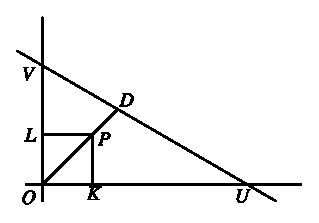
\includegraphics{figures/fig_01.eps}
\end{figure}\pageoriginale
we have at once
$$
OU = - c/a, \quad OV = - c/b, \quad UV = c \surd (a^2 + b^2) /ab;
$$
but the equation in areas,
$$
OPU + OPV + PUV = OUV, 
$$
can now be written
$$
{}-\frac{1}{2} (cy_1/a) - \frac{1}{2} (cx_1 /b) + \frac{1}{2}
PD. c. ~\surd~ (a^2 + b^2) / ab = \frac{1}{2} (c^2/ab)
$$
and from this we derive without further trouble the required length $PD$.

There are of course many variants of this, but the particular instance
given may serve as a text for all of them. It is no doubt elegant,
thought that alone is not enough to convince me of its essential
merit. First, one may comment that the handling of the signs is not
entirely fool-proof, and that the boy who does not draw his line just
as shown may get into serious trouble without knowing why. But the
real objection lies deeper than this. The lure of \textit{ad hoc}
elegance is one which should be firmly resisted in all mathematics,
and perhaps particularly avoided in this field. Will the pupil who has
faithfully followed and absorbed this argument be in any stronger
position when he comes to deal with some similar but slightly
different problem ? Unless he (or she) is very bright indeed, we must
confess that the answer is definitely ``No''. This proof offends
against one of the basic canons of mathematical teaching,  that a
process which does one and only one thing in a very special
way\pageoriginale is not mathematically educative and should be
avoided. Neat tricks and examination tips are in the long run mentally
unsatisfactory and sterile.

\medskip
\noindent
{\textbf{Method III. ~}} In casting about for a more suitable method,
let us begin by asking whether the problem is capable of being
connected with the distance-direction or the distance-ratio idea. The
answer is clear : there is an evident connection with the
distance-direction concept. Very well : let $d$ be the required
distance, and $\alpha$ its direction. The point $D$ will have
coordinates $x_1 + d \cos \alpha$, $y_1 + d \sin \alpha$, and since it
is on the given line $ax + by + c = 0$, we have at once that
$$
a(x_1 + d \cos \alpha) + b (y_1 + d \sin \alpha) + c = 0,
$$
or 
$$
d = - (ax_1 + by_1 + c) / (a \cos \alpha + b \sin \alpha).
$$
We may now identify the trigonometrical functions by observing that
$(-a/b) \tan \alpha = - 1$, but it is to be noticed that this is not a
vital step in the argument, but rather a trivial corollary. We have
solved a problem more general than the one with which we set out, but
this is not a waste of effort ; in a sense, the more general problem
is easier to solve, while the particular result is only a simple
corollary. I will not make any extravagant claim for time-saving,
though I suggest that the possible sources of arithmetic or algebraic
error have been cut down to a minimum. But I do claim that here we
have not had to scratch our heads for a bright idea, we have simply
asked for a connection with out basic principles, have found such a
connection, and then proceeded in a straightforward and almost
inevitable manner. It is hazardous in any branch of mathematics to
claim that any particular proof is the best that can be found, but I
am sure that this is a good and natural proof, depending closely on
basic principles, and that there is much profit to be found in seeking
to link all our proofs to simple fundamentals in this way.

Questions involving the division of a segment are equally clearly
connected with the distance-ratio notion. The ratio in which the
segment joining $P (x_1, y_1)$ to $Q(x_2, y_2)$ is divided by the
straight line\pageoriginale $ax + by + c = 0$ being $h : k$, the point
of division has coordinates $(kx_1 + hx_2) / (h/k)$, $(ky_1 + hy_2)
/(h+k)$, and as this is on the given line, the ratio is at once
determined. I mention this obvious point, however, more for the sake
of a slight digression on conventions of sign ; this problem and the
previous one about the perpendicular distance are frequently made the
excuses for a cloud of obscurity about conventions of sign. It is not
to be denied that sign may be important ; but equally, and here I
quote the distinguished American geometer, Eisenhart, some questions
of sign are important, some are unimportant, and it is part of the
task of the good student to recognise which is which. If the
enthusiasts for sign conventions, here and elsewhere in elementary
mathematics, are asked to justify their verbosities and complexities, 
they so often say, ``Oh, but we must have a convention of sign'', a
dictatorial and dogmatic attitude which arouses my wrath just as it is
aroused by the man who says ``Oh, but we must have another drink''; he
does not need one, he probably does not want one, but he has become
too weak-willed to defy the habit, the convention, of having one more
than he needs or wants. We need not under-estimate the importance of
conventions ; they save a tremendous amount of thought which might
otherwise be wasted on petty details. The normal way of drawing the
axes of $x$ and $y$ is a convention, but it is a good convention
because it can save expenditure of mental energy on small matters ; we
ca build up a general picture of a problem as we read it if our main
conventions are sound and familiar. But the test is pragmatic :
conventions are convenient but not necessary, and the slightly
derogatory flavour about the adjective ``conventional'' clings to it
because we apply it to those who clutch a convention unyieldingly long
after the use on which it was founded has passed away.

In this particular field, there is one simple fact, and we need no
added arbitrary convention. It follows at once from the result about
the division of a segment that the linear forms $ax_1 + by_1 + c$,
$ax_2 + by_2 + c$ have the same sign if $(x_1, y_1)~ (x_2, y_2)$ are
on the same side of the line $ax+by+c=0$, and opposite signs if these
points are\pageoriginale on opposite sides of the line. This is all
that is needed, and there is no merit in cluttering up the matter with
an equipment of conventions as cumbersome and useless as a suit of
armour would be to a channel swimmer. But at this stage, I have
sometimes been faced with what is supposed to be a clinching remark :
``Yes, but how do you find the incentre of a triangle given the
equations of the three sides ?''. My first answer is not intended to
be flippant : I have never yet been in the plight of wanting to find
the iincentre of a triangle given the equations to the three sides,
and I hope that my declining years will never find me wishing to do
anything so stupid. ``Ah, but suppose you did ?'' Well, suppose the
Snark was a Boojum, what then ? The problem is either numerical and
special, or it is general. If it is special, no convention is required
: the simple fact about the division of the plane mentioned above will
serve at once to fix the allocation of signs. But if the problem is
general, then I must be allowed to assert that it is stupid almost
to the length of being meaningless. In the general algebraic geometry
of the plane, the incentre is merely one of a set of four related
points, and the general geometry of the plane has, and can have, no
interest in assigning priority to one of the four over the other
three.


With this simple equipment, most if not all of the coordinate geometry
of the school stage can be elaborated. Once the geometry of the
straight line and the algebra of the linear form have been thoroughly
correlated, there is much to be said for making the next step an
answer to the question. ``What can we discover, by our basic methods,
about the properties of all curves which can be represented by an
equation of the second degree ?'' This is a natural sequel to the
examination of the geometric properties of the linear equation, and
can be much more stimulating than the process, traditional in English
texts, of dealing with special cases in considerable and often
repetitive detail. The degree of sophistication required to appreciate
a moderately general discussion of this type is much less than is
popularly supposed, and such a discussion can easily be comprehended
and found bracing by classes of technicians, as well as by classes of
intending mathematicians.

Calling\pageoriginale the curves `conics' merely for brevity, the intersections of a
straight line with a conic, the tangent at a point on a conic, the
polar, the pair of tangents from a point are all clearly related to
the distance-ratio idea, and the basic results in this field can all
be written down at once when the distance-ratio formula has been made
to yeild Joachimsthal's ratio equation. On the other hand, the study
of parallel chords must be basically related to the distance-direction
concept, and the  application of this leads directly to the discussion
of diameters, existence of a centre, tangents parallel to a given
direction, and related matters. The distinction between central and
non-central conics, and between bounded and unbounded central conics,
fall naturally into place, and separate discussion of the ellipse,
hyperbola and parabola does not begin until the need for it is apparent.

With a technical class, having some professional interest in
draughtsmanship and design, it is instructive and profitable to follow
these ideas up by drawing-board work. The method given by
E. H. Neville (\textit{Mathematical Gazette, 1921}), based on these
general principles, enables us to draw a conic such as 
$$
3x^2 + 4xy - 5y^2 + 6x - 5y + 7 =0 
$$
without the tedious, complicated and unnecessary arithmetic entailed
by the reduction to canonical form and standard axes so often
recommended, and moreover, enables us to draw a conic which looks like
a conic !

I am very conscious that these considerations may seem to be so
elementary as to be unworthy of presentation to this conference ; but
I will make no apology. Here we can and should see the teaching of a
particular topic as an organic whole, form the first steps in the
school to the end of the degree course. Our pupils are more likely to
reach the final stages confidently and successfully if we ensure that
their first steps are in the right direction.

\bigskip
\bigskip

\noindent
{\fontsize{9pt}{11pt}\selectfont
Royal Naval College\\
Greenwich}\relax
